\section{Getting started with FLAMEGPU}\label{sec:hands-on}

To get started with FLAMEGPU, connect to the Amazon instance by following the given instructions in Section~\ref{sec:aws}. Then, download the latest version of FLAMEGPU from GitHub:

%git clone https://github.com/FLAMEGPU/FLAMEGPU.git
\begin{verbatim}
git clone https://github.com/FLAMEGPU/Tutorial.git
\end{verbatim}


A typical top-level directory layout is as below:
%The folder structure of FLAMEGPU is as follows:

\begin{itemize}
\item \textbf{FLAMEGPU:} contains the templates and XML schemas that are used to generate CUDA GPU code. These should not be modified by the users.
\item \textbf{bin/x64} and \textbf{bin/linux-x64:} The location of the console and visualisation binaries for each of the examples. There is a Linux shell script for each example which will start the simulation with an initial states file (and the number of iterations to simulation in console mode)
\item \textbf{doc:} The FLAMEGPU technical report and user guide in addition to reports for specific example models.
\item \textbf{examples:} The location of the model files for FLAMEGPU examples and the location to create your own models.
\item \textbf{include:} Some common include files required by FLAMEGPU
\item \textbf{lib:} Any library dependencies required by FLAMEGPU
\item \textbf{media:} 3D models used for some of the visualisations
\item \textbf{tools:} A number of tools for generating function script files from XML model files and running template code generation in windows.
\end{itemize}

To start with, we are going to work with the predator-prey model (Section~\ref{sec:preypredator}). This is a simple model in which prey agents demonstrate flocking behaviour while moving away from predators. Navigate to the \verb|examples/PreyPredator| directory and call \verb|make|.

\begin{verbatim}
cd examples
cd PreyPredator
make
\end{verbatim}


This will process the XML model and build a console~\footnote{In the original version of FLAMEGPU, calling \textit{make} would build both console and visualisation version of the model in release mode} version of the model in release mode. To run the executable, simply run \verb|make run_console|. Alternatively, navigate back to the FLAMEGPU bin directory and call the \textit{run script} which will have been generated by the make process.

\begin{verbatim}
cd ../../bin/linux-x64/}
./PreyPredator_console.sh
\end{verbatim}

The output will be an XML file (saved in the location of the initial input file) which will contain the state of the agents after applying a single simulation iteration to the agents. You can view this file (via \verb|cat| command) to see how the agent positions and other properties have changed. 


Examine the run script by looking at the parameters passed to the simulation. The parameters are the initial model file and the number simulation runs (iterations). Note that by default, the number of iterations is set to 1. In order to modify the number of iterations, simply pass an argument to the shell script as follows:

\begin{verbatim}
make run_console iter=500
\end{verbatim}

Multiple output files (500 in the above example) will be generated, one for each simulation step~\footnote{By setting the defined macro \textit{OUTPUT\_TO\_XML} to 0, no output file will be generated. The macro is located in \textit{PreyPredator/src/dynamic/main.cu}}. Alternatively, you can use the output of the previous iteration as the input for a new one. For this particular model, we generated the initial data via a simple c++ program. 

\section{Visualising the Model}
Note: This will not work on Amazon AWS images as it is not easily supported. Skip this section for the tutorial unless you are running the examples on your own Ubuntu system~\footnote{Ubuntu users can install VirtualGL and connect to AWS via \textit{vglconnect}. For more info, please refer to their website as this is beyond the scope of this tutorial.}


On your own machine, navigate to the FLAMEGPU bin folder (\verb|bin/linux-x64/|) and run the \textit{vis script} visualisation shell script. This will launch the simulation in visualisation mode. 

You can build the model in visualisation mode rather than console (by default), and then run the executable as follows:

\begin{verbatim}
make Visualisation_mode
make run_vis
\end{verbatim}


\section{Exercise 01}
In exercise one, we are going to build and execute the simulation program for the basic Predator-Prey model, followed by plotting the output results. Navigate to the \verb|examples/PreyPredator| directory.

\begin{verbatim}
cd examples/PreyPredator
make
\end{verbatim}

Now, we run the simulation for 150 iterations:
\begin{verbatim}
make run_console iter=150
\end{verbatim}

The generated output contains the number of prey and predator agents per iteration. The statistical result is stored in iteration folder. Let's navigate to this folder and plot the result:

\begin{verbatim}
cd examples/PreyPredator/iterations/
gnuplot make_plot_PreyPred.gp
\end{verbatim}

You can transfer the \verb|.png| file to your local machine to view it or you can use the \verb|display| command (See Section~\ref{sec:visualisation}). Your plot should be similar to Figure~\ref{fig:simulation_noGrass}. You can observe the predator prey behaviour where both species become extinct after certain number of iterations.


\begin{figure}[!h] 
    \centering
    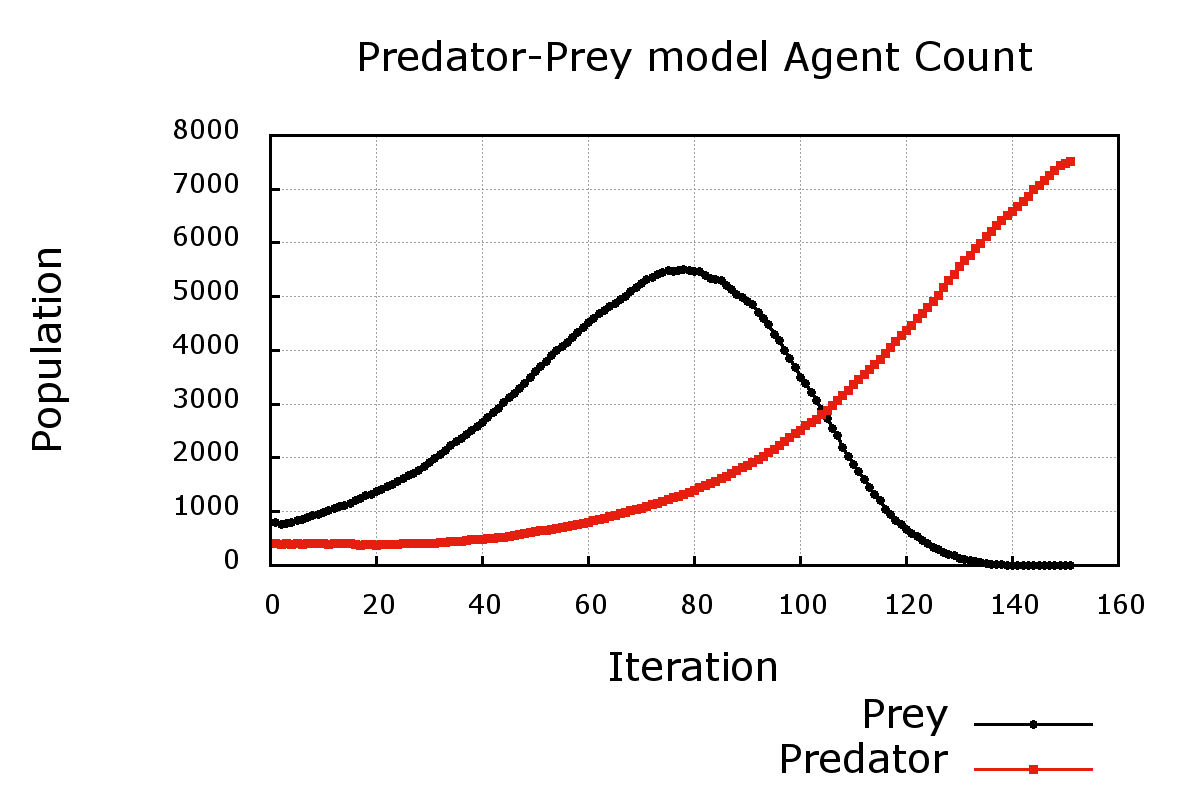
\includegraphics[width=4in]{prey_predator_iter150}
    \caption{Examples of predator-prey model simulation - no grass included (after 150 iteration) }
    \label{fig:simulation_noGrass}
\end{figure}

\section{Exercise 02}
Now, let's change the parameters in the initial data and see how it affects the behaviour. To generate the initial data (0.xml), navigate to \verb|XMLGenerator| folder. 

\begin{enumerate}[{2.1}]
    \item Compile and re-run the executable with different parameters.
%to do
\begin{verbatim} 
cd /examples/PreyPredator/XMLGenerator/
g++ -std=gnu++11 xmlGen.cpp -o xmlGen
./xmlGen ../iterations/0.xml 800 400 0.05 0.03 50
\end{verbatim}
, where 800 is the number of predators, 400 is the number of preys, 0.05 and 0.03 are the reproduction rates for both prey and predator, and 50 is the predator's energy gain. 


\item Re-run the executable again for 300 iterations and plot the results. Your plot should be similar to Figure~\ref{fig:simulation_noGrass_exr2}.

\begin{figure}[!h]
    \centering
    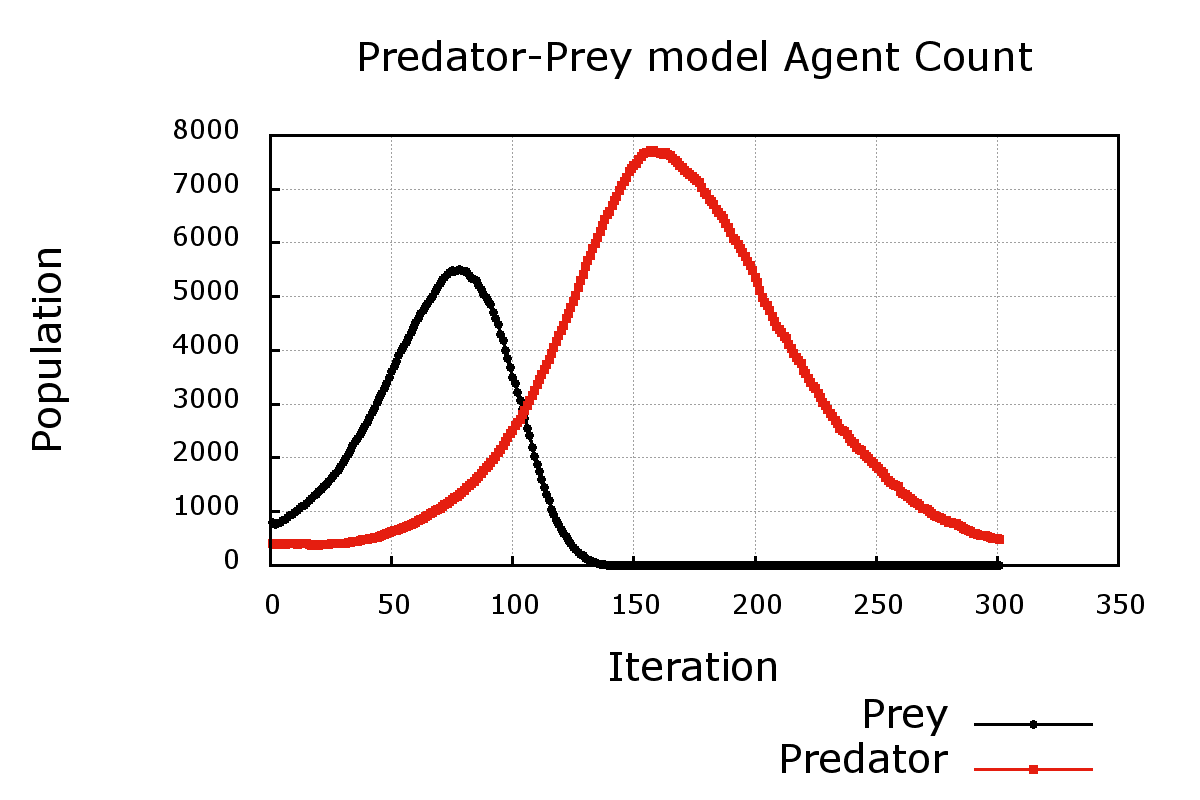
\includegraphics[width=4in]{prey_predator}
    \caption{Examples of predator-prey model simulation - no grass included (after 300 iteration)}
    \label{fig:simulation_noGrass_exr2}
\end{figure}

\item Change the other parameters or the iteration number to see how the behaviour changes.
\end{enumerate}
\section{Exercise 03}
In this exercise, we are going to extend our model to include grass. We have previously described the behaviour of the model when grass included. Agent grass description has already be added to the XML model file. In this exercise, you need to modify \verb|function.c| file to include below functions:

\begin{enumerate}[{3.1}]
\item \textbf{grass\_output\_location}: each grass agent outputs information to be read by other agents
\item \textbf{grass\_eaten}: each grass agent iterates over \verb|prey_location_messages| and checks the distance between its location and the prey agent. If the grass is available and the distances less than \verb|GRASS\_EAT\_DISTANCE|, then the grass is eaten by the closet prey and the regrowth cycle starts. Note that if there are multiple preys within the \verb|GRASS\_EAT\_DISTANCE|, then the closet prey to the grass, eats it and outputs a message \verb|grass_eaten| containing the ID of the prey who ate it.

Once the grass is eaten, its colour changes (\verb|type| variable is set to a different colour) and it no longer will be available until the \verb|death_cycles| reaches \verb|GRASS_REGROW_CYCLES|). 
\item \textbf{prey\_eat\_or\_starve}: each grass agent iterates over \verb|grass_eaten_messages| and checks the ID against it ID. If the grass eaten message indicates that this prey ate some grass then increase the preys life by adding energy. Moreover, if its life is less than 1, it dies.
\item \textbf{grass\_growth}: If the the \verb|death_cycles| variable is equal to \verb|GRASS_REGROW_CYCLES|, then the grass agent becomes available and the \verb|death_cycles| restarts and the colour will be set to green again. If the grass is not available (meaning the \verb|death_cycles| variable is not equal to \verb|GRASS_REGROW_CYCLES|), then we only increase the \verb|death_cycles| variable.
\end{enumerate}


Now, generate a new initial data file using below parameters. Then re-build the model via \verb|make| and run the simulation for 600 iterations \verb|make run_console iter=600|. Your plot should be similar to Figure~\ref{fig:simulation_Grass}.

\begin{verbatim}
cd /examples/PreyPredator/XMLGenerator/
g++ -std=gnu++11 xmlGen_IncGrass.cpp -o xmlGen
./xmlGen ../iterations/0.xml 800 400 2000 0.05 0.03 75 50 100
\end{verbatim}

, where 800 is the number of preys, 400 is the number of predators, 2000 is the number of grass, 0.05 and 0.03 are the reproduction rates for both prey and predator, 75 is the prey's energy gain, and 50 is the predator's energy gain. 


\begin{figure}[!h]
    \centering
    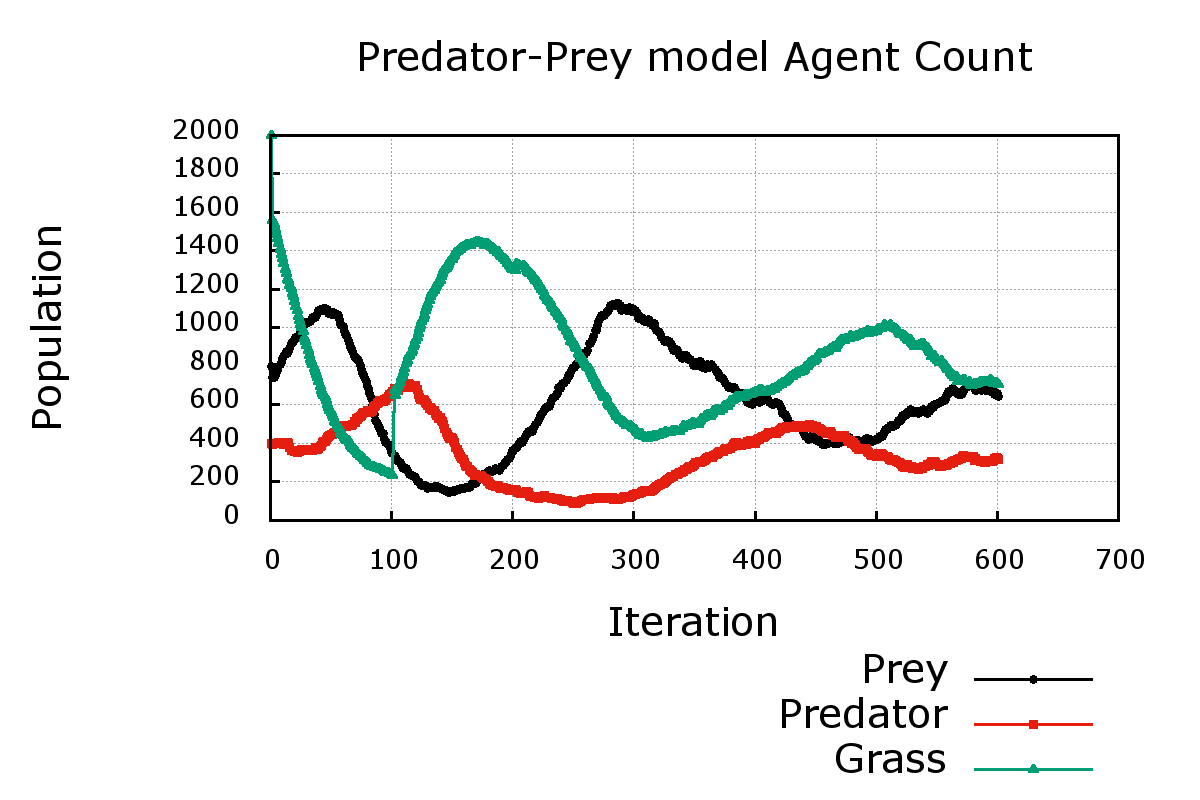
\includegraphics[width=4in]{prey_predator_grass}
    \caption{Examples of predator-prey model simulation with grass included}
    \label{fig:simulation_Grass}
\end{figure}

\section{Experimenting with the Model}
Try changing the parameters to see how this will change the behaviour of the agents causing the behaviours to change.

For more information on FLAMEGPU see the FLAMEGPU website\footnote{www.flamegpu.com} and the documentation which gives detailed instructions on all aspects of FLAMEGPU modelling. More examples can be found on FLAMEGPU GitHub repository (\verb|https://github.com/FLAMEGPU/FLAMEGPU.git|).

You can download the solutions from GitHub (\href{https://github.com/FLAMEGPU/tutorial/}{https://github.com/FLAMEGPU/tutorial/}).
